\secput{meta}{Introduction to meta-algorithm} 
% introduction to meta-algorithm, the basic notion: take one algorithm as 
% input and output another algorithm which is asymptotically better, along 
% with application in orthogonal range queries 

\subsecput{intro-meta}{Introduction to meta-algorithms and its application
to $2$-D orthogonal range queries}

In \cite{Yao82, Yao85}, A. Yao introduced an algorithm to preprocess
a $1$-D grid recursively in $O(n \alpha(n))$ space and time bound and
answer later online range queries in time $O(\alpha(n))$. A
good graphical illustration of how the algorithm works can be found
in \cite{Seidel06}. Yao's algorithm \cite{Yao82,
Seidel06} can be viewed as $1$-D meta-algorithm as defined below.
We call an algorithm a \defn{meta-algorithm} if it
takes an algorithm (called an \defn{initial algorithm}) as input, 
applies it as a black box on some
manipulated version of the input data, and effectively behaves
like a new algorithm with different (ideally improved) asymptotic 
performance bounds. The idea similar to that of a higher-order 
function in a functional language.

In this section, we demonstrate how to use the notion of meta-algorithms
to process $2$-D orthogonal range queries. Extension to higher-dimensional
grids is similar and omitted from this extended abstract due to
space limitations. In \secref{poly} we will show
how to extend it to support non-orthogonal range queries, such as triangular
and polygonal queries in $2$-D grids.

\subsubsecput{init-2D}{Initial algorithm for $2$D grids}

\punt{%
\begin{figure*}[!ht]
\centering
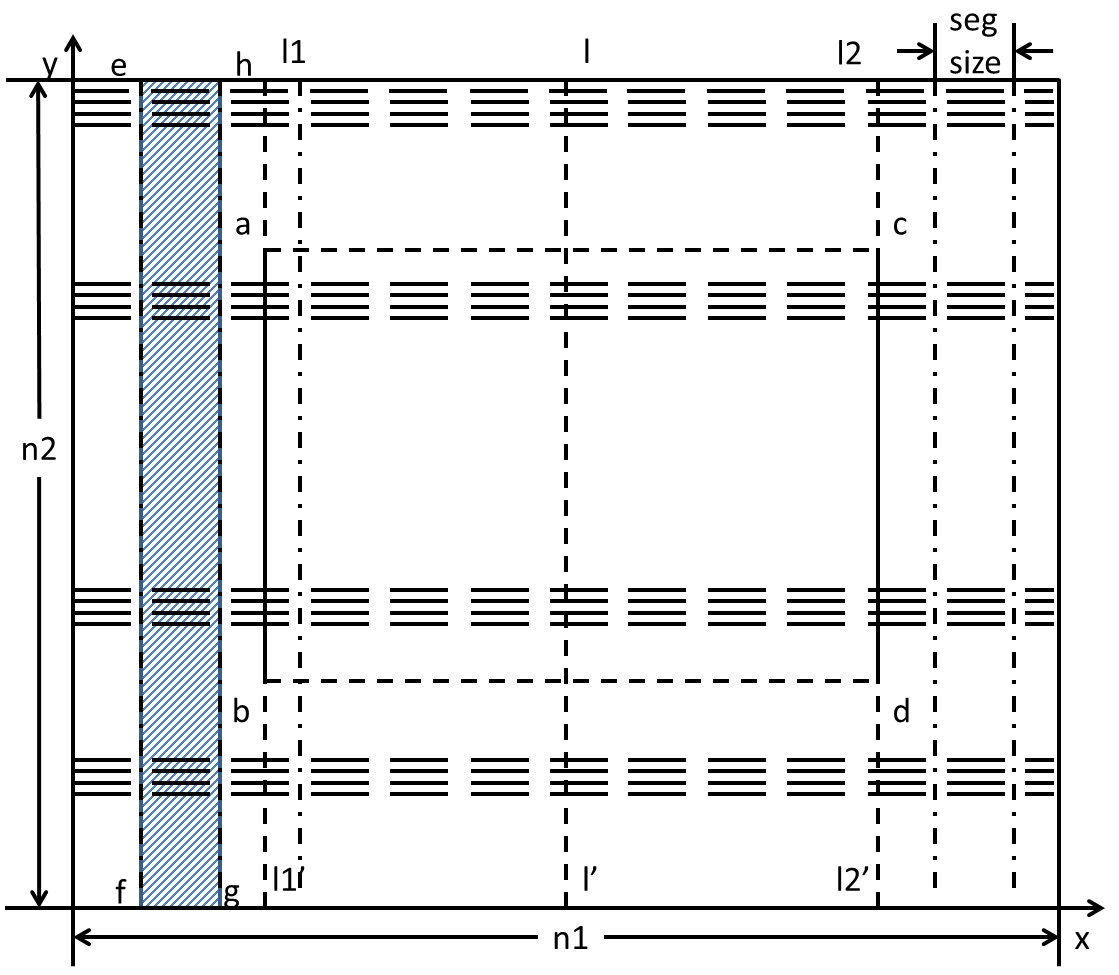
\includegraphics[clip,width=3in]{figures/meta_2D.eps}
\vspace{-1cm}
\caption{Meta-algorithm for $2$D orthogonal range queries}
\label{fig:meta-2D}
\end{figure*}
} %\end punt

First we need an initial algorithm to kick off. The initial algorithm 
does not need to be very efficient as long as it solve the problem
correctly. Our meta-algorithm only needs to know the complexity
bound of the initial input algorithm, but no knowledge
of any internal data structure or the internal workings
of the algorithm is needed. 
%
One such algorithm is given in \figref{init-2D-algo} of
\secref{apdx-init-2D}. 
%
The preprocessing time and space of this initial $2$-D 
algorithm $\Theta(N \log^2 N)$ for a grid of size $N$,
and the query overhead is only 3 semigroup operations. 


\punt{%
\begin{enumerate}
\item Select a longer dimension, without loss of generality, let's
  suppose it's dimension $\id{x}$.
\item Partition dimension $\id{x}$ by a center line $\overline{\id{ll'}}$
  into evenly two parts. Then all points in the grid resides
  either on the left (e.g.  $\id{p_1}$) of the center line or right
  (e.g. $\id{p_2}$). For all the points, reducing (by applying the $\oplus$
  operator) the data from center line to itself by dynamic programming.
  We call the reduced data prefix or suffix value from the center line.
\item After data reduction on both prefix and suffix values, applying Yao's
  initial $1$-D preprocessing algorithm \cite{Yao82, ChazelleRo91},
  which has complexity $O(n \log (n))$ on all lines along vertical
  dimension $\id{y}$.
\item Now we have the observation that all $2$-D orthogonal range query
  that spans across the center line $\overline{\id{ll'}}$ can be
  answered by conducting two $1$-D queries on both left-hand side
  and right-hand side of the center line. E.g. To query the rectangle
  $\Box\id{abdc}$ in \figref{init-2D}, we perform one $1$-D query
  on line $\overline{\id{l_1l_1'}}$ and another $1$-D query on line
  $\overline{\id{l_2l_2'}}$. Combining these two results by $\oplus$
  operator, we get the final query result of the orthogonal range query.
\item Recursively applying the above procedure to the left and right
  sub-grids of line $\overline{\id{ll'}}$ completes the initial algorithm
  and covers all possible range queries in the grid.
\end{enumerate}

\begin{theorem}
The preprocessing of this initial $2$-D algorithm has complexity of
$\Theta(n_1 n_2 \log (n_1) \log(n_2))$ in both time and space. 
\label{thm:init-2D-pp}
\end{theorem}

\begin{corollary}
The query overhead of this initial $2$-D algorithm is $3-\oplus$. 
\label{cor:init-2D-query}
\end{corollary}
}
% punt ends


\subsubsecput{meta-2D}{Meta-algorithm for $2$D grids}

The meta-algorithm takes one initial algorithm as input, compresses the
data alternatively along dimension $\id{x}$ or $\id{y}$ to eventually hit
the alpha bound. The description follows the notation in \figref{meta-2D}
and the pseudo-code in \figref{meta-2D-algo}.
(\figref{meta-2D} is also a graphical illustration of how the algorithm
 works) 

\begin{enumerate}
\item We start data reduction on a longer dimension,
  w.l.o.g., suppose it's dimension $\id{x}$. For
  each line of dimension $\id{y}$, partition it along dimension
  $\id{x}$ into segments of size $\id{seg\_size}$,
  which is $f_{1}(n_1)$ assuming that
  the complexity of the input algorithm ($\id{input\_2D\_algo}$) 
  is $\Theta(n_1 n_2 f_1(n_1) f_2(n_2))$.
%
\punt{
$\log (\id{x_1} - \id{x_0})$, or
  $\log^* (\id{x_1} - \id{x_0})$, $\log^{**} (\id{x_1} - \id{x_0})$,
  $\ldots$ ($\id{seg\_size}$ in \figref{meta-2D-algo}). The length of
  $\id{seg\_size}$ depends on the complexity of $\id{input\_2D\_algo}$,
  which can be a user's input parameter.
}
% punt ends
\item Apply the $\oplus$ operator to reduce
  all data within each segment into a single value. All such values
  construct a new grid --- $\id{promoted\_grid}$. Apply
  $\id{input\_2D\_algo}$ on $\id{promoted\_grid}$.
%
\item For each vertical line (along dimension $\id{y}$), reduce the
  the data relative to the left and right end of each segment (of
  size $\id{seg\_size}$) to construct $\id{prefix\_grid}$ and
  $\id{suffix\_grid}$.
%
\item For each vertical line (e.g. line $\overline{l_1l_1'}$ and
  line $\overline{l_2l_2'}$ in \figref{meta-2D}) in $\id{prefix\_grid}$
  and $\id{suffix\_grid}$, apply the $\id{input\_1D\_algo}$ on it.
  If the $\id{input\_2D\_algo}$ has bound $\Theta(n_1 n_2 f_1(n_1)
  f_2(n_2))$, the corresponding $\id{input\_1D\_algo}$ should have a bound of
  $\Theta(n f(n))$, where $f(n) \leq f_1(n)$ and $f(n) \leq f_2(n)$.
  Otherwise though the meta-algorithm will still be correct
  it won't have the desired performance bounds.
%
\item Recursively apply the meta-algorithm on segment blocks
  of size $\id{seg\_size} \times \id{n_2}$, e.g., on the colored segment block 
  $\Box \id{efgh}$ in \figref{meta-2D}.
%
\item Apply the meta-algorithm described above alternatively on dimensions
  $\id{y}$ and $\id{x}$.
%
\end{enumerate}

\begin{theorem}
Given an input $2D$ algrithm with a preprocessing complexity (in both space and time)
of $\Theta(n_1 n_2 f(n_1) f(n_2))$, where $f(n) \leq n-2$,
one round of application of the meta-algorithm
reduces the bound to $\Theta(n_1 n_2 f^*(n_1) f^*(n_2))$.
\label{thm:meta-2D-pp}
\end{theorem}

\begin{corollary}
Given an input $2D$ algrithm with a preprocessing complexity (in space and time)
of $\Theta(n_1 n_2 f(n_1) f(n_2))$, where $f(n) \leq n-2$,
and a constant query overhead,
$O(\alpha(n_1)\alpha(n_2)$ rounds of application of the meta-algorithm
reduces the preprocessing bound to $\Theta(n_1 n_2 \alpha(n_1) \alpha(n_2))$
at the cost of increasing the the query overhead to
$\Theta(\alpha(n_1)\alpha(n_2))$.
\label{cor:meta-2D-query}
\end{corollary}

More technical details, including pseudo-codes, proofs of theorems 
and corollaries, can be found in \secref{apdx-meta-intro}.
